\renewcommand*{\arraystretch}{1.1}

\noindent\begin{tabularx}{17cm}{|>{\small \sf}c|X|}
	\hline
	query    & Interactive / update / 4 \\ \hline
%
	title       & Add Forum \\ \hline
%
    pattern     & \hfill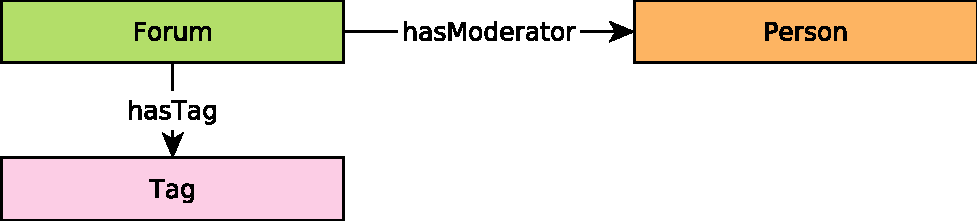
\includegraphics[scale=\patternscale,margin=0cm .2cm]{patterns/interactive-update-04}\hfill\vadjust{} \\ \hline
%
	desc. & Add a Forum to the social network.
 \\ \hline
%
	
%
	params.  &
	\vspace{1.1ex}{\begin{tabularx}{14.66cm}{|c|M|m{2cm}|Y|} \hline
	\cellcolor{parameter} \color{white} $\mathsf{1}$ & \varname{Forum.id} & \cellcolor{gray!20} \vartype{ID} &  \\ \hline
	\cellcolor{parameter} \color{white} $\mathsf{2}$ & \varname{Forum.title} & \cellcolor{gray!20} \vartype{String} &  \\ \hline
	\cellcolor{parameter} \color{white} $\mathsf{3}$ & \varname{Forum.creationDate} & \cellcolor{gray!20} \vartype{DateTime} &  \\ \hline
	\cellcolor{parameter} \color{white} $\mathsf{4}$ & \varname{Forum-hasModerator->Person.id} & \cellcolor{gray!20} \vartype{ID} &  \\ \hline
	\cellcolor{parameter} \color{white} $\mathsf{5}$ & \varname{Forum-hasTag->Tag.id} & \cellcolor{gray!20} \vartype{\{ID\}} &  \\ \hline
	\end{tabularx}}\vspace{1.1ex} \\ \hline
%
	
%
	%
	%
	%
    %
\end{tabularx}
\vspace{2ex}